\section{Research-harness evolution}
\label{sec:harness}

The continuation loop adapts a harness through a bounded sequence of Propose--Probe--Compose decisions. At decision $t$, a proposer receives the current harness and its permitted information packet, then returns one atomic proposal $e_t$ containing two to five edits. The operator $A$ applies the complete array to the current harness and validates the resulting operator roster:
\begin{equation}
H_t^{c}=A(H_{t-1},e_t).
\label{eq:atomic}
\end{equation}
The array therefore represents one composite harness candidate. Earlier JSON arrays with independent-edit semantics retain their historical meaning and are not reinterpreted in the present protocol.

Probe execution evaluates the candidate under the current task contract and produces factor-expression candidates, behavioral measurements, and execution traces. The active branch carries the continuation state into the next decision even when an edit is not adopted. A frozen champion changes only when the task contract is satisfied. This separation allows exploration to continue without turning every temporary improvement into the final evaluated object.

Figure~\ref{fig:method} summarizes the information flow. Historical probe memory excludes select outcomes. Online execution remains probe-only, and one frozen champion per condition enters the final comparison. All relevant candidates and parent signals are evaluated on their common \texttt{date+symbol} support, so paired contrasts do not combine estimates computed on different samples.

\begin{figure*}[!htbp]
\centering
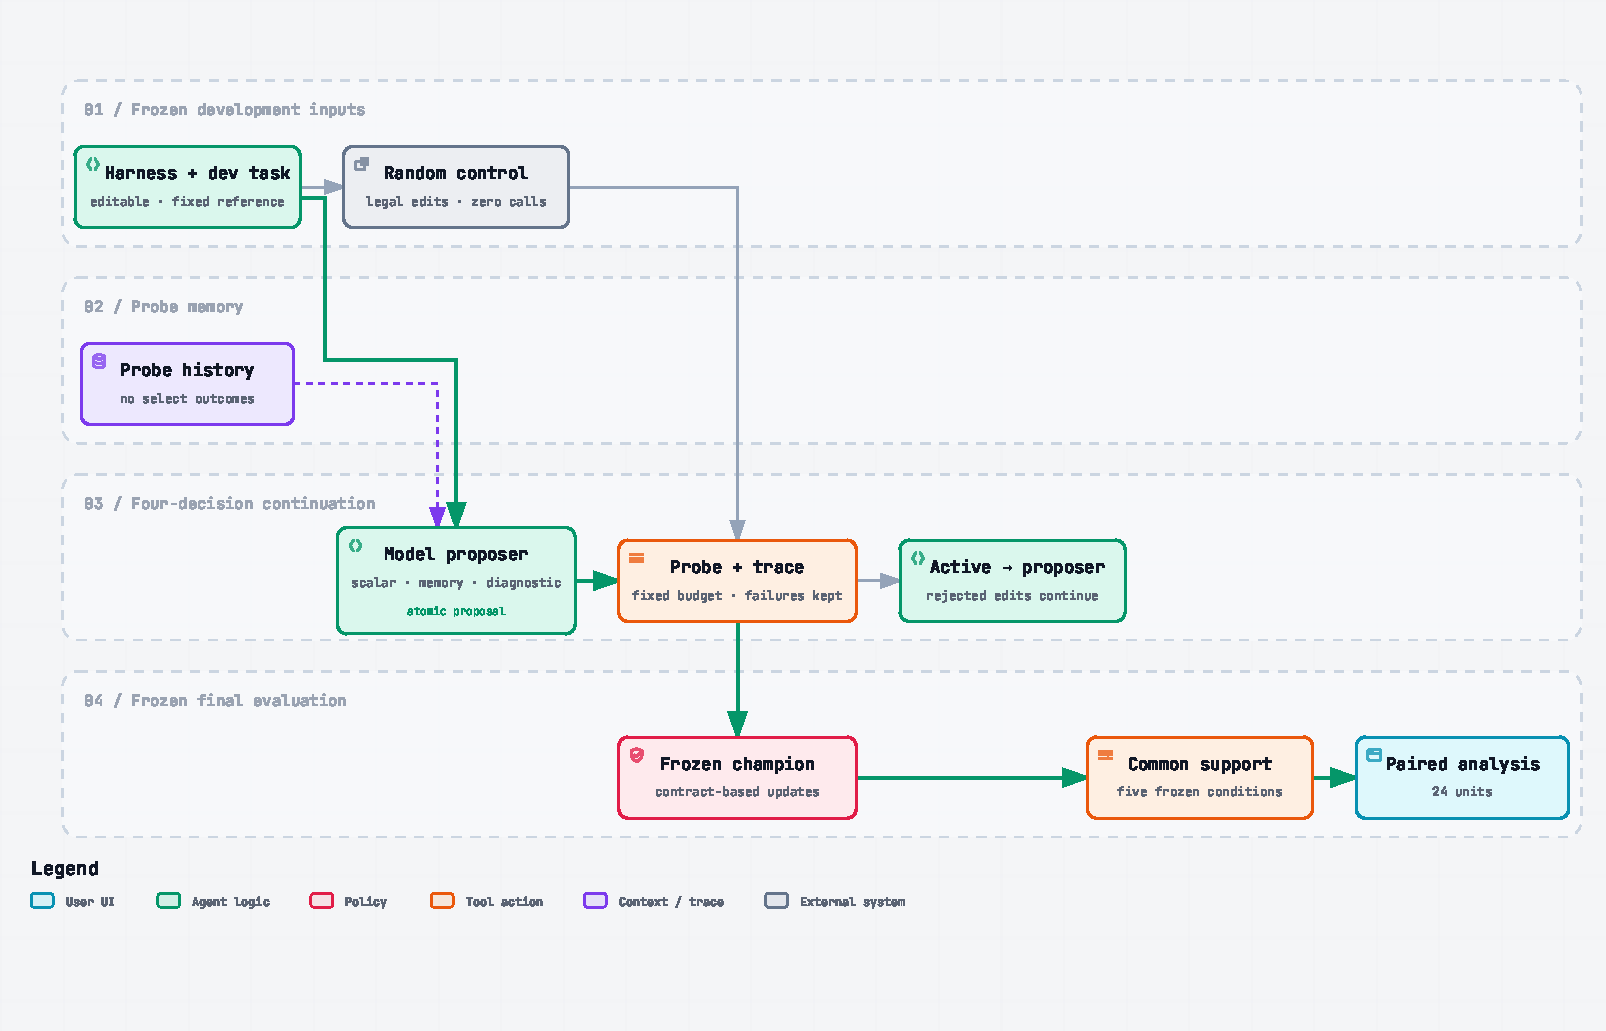
\includegraphics[width=\ResearchWideWidth]{figures/figure_01_method_pipeline.pdf}
\caption{Budget-bounded research-harness continuation and evaluation. Scalar, cumulative-memory, and diagnostic proposers emit one atomic proposal per decision; random legal edits use zero model calls. Probe execution feeds a four-decision active branch and one frozen champion per condition, followed by the final common-support comparison. The diagram also marks the fixed candidate budget, retained failures, and exclusion of select outcomes from historical probe memory.}
\label{fig:method}
\end{figure*}

The random backend reads the same current harness and editable surface and produces legal atomic proposals without a model call. The fixed reference evaluates the unchanged initial harness. These references distinguish model-guided adaptation from random legal edits over the same editable surface and from the initial research process. Within this fixed process, scalar feedback, cumulative memory, and compact diagnostics form the separable information conditions.
